\chapter{Methodik}\label{ch:methodik}
In diesem Kapitel wird näher erläutert, warum und welche Daten für das Experiment in \autoref{ch:experimentundergebnis} ausgewählt wurden. Außerdem wird darauf eingegangen, inwiefern die Daten vorbereitet wurden und mit welchen Parametern die Verfahren gestartet und ausgewertet wurden.

\section{Datenbasis}
Für das Experiment wurden drei verschiedene Datensätze benutzt, die drei verschiedene Fälle abdecken: 
\begin{itemize}
    \item der Aktienkurs von Nvidia \cite{nvidiaStock}, wobei hier die Differenz zwischen Schlusskurs und Eröffnungskurs genutzt wird,
    \item die tägliche Durchschnittstemperatur an Wetterstationen in Europa \cite{ecadWetterdaten},
    \item ein EKG \cite{ecg500}, wobei hier der Datensatz \textit{ECG5000\_TRAIN.txt} genutzt wird.
\end{itemize}

Aktienkurse sind interessant, da man in Ihnen Trends erkennen kann oder sogar Saisonalität, also z.~B. dass der Kurs zum Jahresende immer steigt, weil wegen Weihnachten der Umsatz steigt. Ansonsten ist die Struktur der Daten unorganisiert, heißt die Daten rauschen viel und es kann extreme Sprünge geben.

Die Wetterdaten sind von verschiedenen Wetterstationen aus ganz Europa und sollen dadurch verschiedene Klimas abdecken. Wegen der Jahreszeiten lassen sich somit die Daten gut bezüglich ihrer Saisonalität vergleichen, besser als bei Aktienkursen. Allerdings sind weniger Trends zu erkennen, da diese über längere Perioden geschehen, als wir sie betrachten. Die Struktur von Wetterdaten ist sehr glatt, bis auf die Schwankungen zwischen den Jahreszeiten sind die Verläufe sehr stetig.

Die EKG"=Daten wiederum sind interessant, weil sie weder Saisonalität noch Trends bieten, dafür eine sehr strenge Struktur haben. Sie wiederholen sich in einer sehr kleinen Periode und haben eine feste Wellenform, von der nur bei bestimmten Ereignissen abgewichen wird.
\section{Vorverarbeitung}
Die Datensätze müssen für die Weiterverarbeitung nach dem Herunterladen vorbereitet werden, denn sie enthalten nicht nur die Werte, die wir brauchen, sondern auch Zeitstempel, Beschreibungen der Daten und weitere Zusätze. Um die Nachprüfbarkeit des Experiments zu erleichtern und um selbst schneller die Daten nutzen zu können, übernimmt das Skript, das zum Teil in \autoref{lst:dataPreparation} erwähnt wird, diese Aufgabe.

Aufgabe dieses Skripts ist allgemein nur die Werte herauszufiltern, die für das Experiment von Relevanz sind. Das wäre beim Aktienkurs die Kursdifferenz und bei den Wetterdaten die Durchschnittstemperatur. Der EKG"=Datensatz beinhaltet bereits lediglich die Messwerte. 

Des Weiteren nimmt das Skript noch weitere, spezifischere Schritte vor. Die Zeitreihe des Aktienkurses wird in weitere Zeitreihen mit nur 50 Werten aufgeteilt, so dass später der Aktienkurs in Abschnitten von 50 Tagen analysiert werden kann. Diese neuen Zeitreihen werden dann in Dateien mit den Namen \textit{50.csv, 100.csv, 150.csv, \dots} geschrieben. Die Wetterdaten enthalten für jeden Tag einen \textit{Quality Code}, der entweder 0 (valide), 1 (auffällig) oder 9 (fehlt) ist. Wetterstationen, die an einem oder mehreren Tagen einen \textit{Quality Code} ungleich 0 haben, werden komplett ignoriert und nicht weiter verwendet. Unter den übrig gebliebenen werden die aussortiert, die weniger als 1000 Messwerte haben, da die letzten 1000 Tage jeder Wetterstation zur späteren Analyse verwendet werden. Die neuen Zeitreihen haben dabei denselben Dateinamen wie die vorherigen, lediglich die Endung ändert sich zu \text{.csv}. Bei den EKG"=Daten befinden sich alle Herzschläge in einer Zeitreihe, für unser Vorhaben müssen diese allerdings, wie der Aktienkurs auch, in mehrere aufgeteilt werden. So wird jeder Herzschlag, also 140 Werte, in eine neue Zeitreihe gepackt. Diese neuen Zeitreihen werden dann in Dateien mit den Namen \textit{140.csv, 280.csv, 420.csv, \dots} geschrieben.
\section{Kompression und Analyse}
Zur Kompression und Analyse sind gewisse Parameter einzustellen: einerseits um unterschiedliche Kompressionsraten zu erzielen, andererseits um einen bestimmten Prozentsatz an Ausreißern zu erkennen oder um einen Schwellwert für die Ausreißererkennung festzulegen.

\begin{table}[b]
 \centering
 \begin{tabular}{lc|cccc}
  \toprule
  \multicolumn{1}{c}{\bfseries Daten} & \boldmath $\rho$ & \bfseries Linear & \bfseries Polynomiell & \bfseries Fourier & \bfseries Wavelet \\
  \midrule
  \multirow{3}{*}{Wetterdaten} & 0,50 & \tabledata{15}{32}{15}{3}
  & 0,25 & \tabledata{35}{75}{5}{4}
  & 0,10 & \tabledata{95}{200}{2}{6}
  \midrule
  \multirow{3}{*}{NVIDIA-Aktie} & 0,50 & \tabledata{5}{9}{100}{1}
  & 0,25 & \tabledata{9}{20}{30}{2}
  & 0,10 & \tabledata{30}{50}{1}{4}
  \midrule
  \multirow{3}{*}{ECG5000} & 0,50 & \tabledata{7}{15}{50}{2}
  & 0,25 & \tabledata{14}{30}{20}{3}
  & 0,10 & \tabledata{35}{100}{8}{4}
  \bottomrule
 \end{tabular}
 \caption{Parameter zur Kompression}
 \label{tbl:metrikenKompression}
\end{table}

Der im Folgenden verwendete Begriff der Kompressionsrate $\rho$ ist in \cite[Ch. 3.3]{compressionSurvey} als $\rho = \frac{s'}{s}$ definiert, wobei $s'$ die komprimierte Größe der Zeitreihe ist und $s$ die Größe der originalen Zeitreihe. Um die späteren Analysen auf verschieden stark komprimierten Daten zu testen, haben wir uns für drei Kompressionsraten entschieden. Gewählt wurden 50\%, 25\% und 10\% der ursprünglichen Dateigröße. Die beiden größeren Zielgrößen orientieren sich an typischen Anwendungsfällen aus der Praxis, wohingegen die kleinste Zielgröße der Analyse eines Extremfalls dient. In \autoref{tbl:metrikenKompression} sieht man die Parameter der Kompressionsverfahren, die in ihrer aufgeführten Reihenfolge an das Skript aus \autoref{lst:surveyExecution} übergeben werden müssen, um die gewünschten Kompressionsraten zu erzielen.

Die tatsächliche Kompressionsrate einer Zeitreihe wurde anhand der Text"=Dateigröße in Bytes ermittelt. Vorteilhaft an dieser Herangehensweise ist, dass man den tatsächlichen Speicherverbrauch betrachtet, der in der Praxis der relevante Wert beim Komprimieren ist. Nachteilhaft ist allerdings, dass man nur begrenzt Rückschlüsse auf den Informationsgehalt der komprimierten Zeitreihe. Damit ist gemeint, dass zwei Zeitreihen zwar gleich viele Werte haben können, sich ihr Platzbedarf jedoch unterscheidet: besitzen die Werte der einen Zeitreihe nur eine Nachkommastelle, so benötigt sie weniger Platz als eine Zeitreihe, deren Werte mit mindestens zehn Nachkommastellen gespeichert werden. 

\begin{table}[t]
 \centering
 \begin{tabular}{lc|ccccc}
  \toprule
  \multicolumn{1}{c}{\bfseries Daten} & \boldmath $\rho$ & \bfseries Original & \bfseries Linear & \bfseries Polynomiell & \bfseries Fourier & \bfseries Wavelet \\ 
  \midrule
   \multirow{3}{*}{Wetterdaten} & 0,50 & \multirow{3}{*}{1000} & \tabledata{134}{128}{310}{125}
   & 0,25 & & \tabledata{58}{56}{141}{63}
   & 0,10 & & \tabledata{22}{20}{89}{16}
   \midrule
   \multirow{3}{*}{NVIDIA-Aktie} & 0,50 & \multirow{3}{*}{\phantom{00}50} & \tabledata{20}{24}{25}{25}
   & 0,25 & & \tabledata{12}{12}{25}{13}
   & 0,10 & & \tabledata{4}{4}{25}{4}
   \midrule
   \multirow{3}{*}{ECG5000} & 0,50 & \multirow{3}{*}{\phantom{0}140} & \tabledata{40}{40}{70}{35}
   & 0,25 & & \tabledata{20}{20}{56}{18}
   & 0,10 & & \tabledata{8}{8}{17}{9}
  \bottomrule
 \end{tabular}
 \caption{Anzahl der durchschnittlichen Double"=Werte}
 \label{tbl:kompressionsratenDoubleWerte}
\end{table}
\begin{table}[t]
 \centering
 \begin{tabular}{lc|ccccc}
  \toprule
  \multicolumn{1}{c}{\bfseries Daten} & \boldmath $\rho$ & \bfseries Original & \bfseries Linear & \bfseries Polynomiell & \bfseries Fourier & \bfseries Wavelet \\ 
  \midrule
   \multirow{3}{*}{Wetterdaten} & 0,50 & \multirow{3}{*}{4543} & \tabledata{2565}{2641}{2629}{2436}
   & 0,25 & & \tabledata{1131}{1181}{1052}{1196}
   & 0,10 & & \tabledata{427}{427}{575}{310}
   \midrule
   \multirow{3}{*}{NVIDIA-Aktie} & 0,50 & \multirow{3}{*}{1103} & \tabledata{445}{540}{518}{554}
   & 0,25 & & \tabledata{267}{273}{247}{287}
   & 0,10 & & \tabledata{88}{91}{138}{86}
   \midrule
   \multirow{3}{*}{ECG5000} & 0,50 & \multirow{3}{*}{1702} & \tabledata{818}{877}{848}{651}
   & 0,25 & & \tabledata{405}{440}{480}{362}
   & 0,10 & & \tabledata{163}{176}{169}{178}
  \bottomrule
 \end{tabular}
 \caption{Durchschnittliche Dateigröße in Bytes}
 \label{tbl:kompressionsratenBytes}
\end{table}

Während in der \autoref{tbl:kompressionsratenBytes} die Dateigrößen einer Zeitreihe in Bytes zu finden sind, sind in \autoref{tbl:kompressionsratenDoubleWerte} die Anzahl der Double"=Werte einer Zeitreihe zu finden. Die Double"=Werte sind dazu da, den Informationsgehalt der Zeitreihen zu bewerten und Rückschlüsse darauf ziehen zu können, wie viel Platz eine Zeitreihe in Form eines Arrays verbrauchen würde. Die Werte in \autoref{tbl:kompressionsratenDoubleWerte} und \autoref{tbl:kompressionsratenBytes} sind über alle Zeitreihen einer Kategorie (Original, Linear"=approximiert, \dots) gemittelt und gerundet. In \autoref{tbl:kompressionsratenBytes} fällt auf, dass mit der Wavelet"=Transformation nicht immer exakt die Kompressionsraten erreicht werden konnten. Das hängt damit zusammen, dass die Anzahl der Werte immer nur halbiert werden kann und somit keine beliebigen Kompressionsraten realisierbar sind. Aus demselben Grund, aus dem wir die Anzahl der Double"=Werte angeben, entspricht eine Halbierung der Double"=Werte nicht zwangsläufig einer Halbierung der Text-Dateigröße. Bei den anderen Kompressionsverfahren wurde versucht, zwei Bedingungen bestmöglich zu erfüllen, und zwar dass die eigentliche Kompressionsrate erreicht wird und man gleichzeitig nicht allzu weit weg von der tatsächlichen Kompressionsrate der Wavelet"=Transformation ist.

Bei den Ausreißererkennungsverfahren wurden keine eigenen Parameter gesetzt, sondern die Standardwerte der jeweiligen Funktionen übernommen. Das hat vor allem zwei Gründe, einerseits sind die gesetzten Parameter etablierte Standardwerte, die auch in \autoref{ch:theoretischegrundlagen} bei den jeweiligen Verfahren genannt werden, andererseits liegt der Fokus der Arbeit darauf, wie gut die Analyseverfahren die vermeintlichen Ausreißer in den originalen Daten auch in den komprimierten Daten finden. Ob diese Daten tatsächlich Ausreißer sind, ist dafür nicht relevant. Bei dem Verfahren für Ähnlichkeitssuche muss hingegen angegeben werden, wie viele nächste Nachbarn man zurückgeben möchte. In unserem Fall haben wir diesen auf 100 gesetzt, denn ein zu kleiner Wert wäre zu anfällig für Rauschen, also dass ein paar wenige Werte in den komprimierten Daten nicht mehr als Nachbarn erkannt werden, und ein zu großer Wert verliert an Sinnhaftigkeit, da sich dann die Daten zu stark unterscheiden und nicht mehr "`ähnlich"' sind.
\section{Auswertung}\label{sec:auswertung}
\newcommand{\tikztextc}[3]{\node at (#1, #2) {\vphantom{/}\smash{#3}};}
\newcommand{\tikztextupc}[3]{\node at (#1, #2) [rotate = 90] {\vphantom{/}\smash{#3}};}
\definecolor{myRed}{RGB}{255, 119, 94}
\definecolor{myGreen}{RGB}{140, 255, 144}
Zur Auswertung, wie gut ein Analyseverfahren abgeschnitten hat, wurden zwei Klassifizierungen vorgenommen. Einmal wurden die tatsächlichen Ausreißer und Nachbarn markiert -- also die, die auf den originalen Zeitreihen erkannt wurden -- und einmal wurden die vorhergesagten Ausreißer und Nachbarn markiert -- also die, die auf den komprimierten Zeitreihen erkannt wurden. Nachdem alle Zeitreihen klassifiziert waren, konnte eine sogenannte Konfusionsmatrix erstellt werden, die Grundlage für häufig genutzte Metriken ist \cite{konfusionsmatrix}. \autoref{fig:konfusionsmatrix} zeigt wie eine solche Konfusionsmatrix aussieht. Die Klassifizierungen führen zu vier Fällen: \begin{enumerate}
    \item die Anzahl der Zeitreihen, die in den originalen und komprimierten Zeitreihen markiert wurden, zählen zu richtig positiv (engl. \textit{\textbf{T}rue \textbf{P}ositive}),
    \item die Anzahl der Zeitreihen, die nicht in den originalen aber in den komprimierten Zeitreihen markiert wurden, zählen zu falsch positiv (engl. \textit{\textbf{F}alse \textbf{P}ositive}),
    \item die Anzahl der Zeitreihen, die nicht in den originalen und nicht in den komprimierten Zeitreihen markiert wurden, zählen zu richtig negativ (engl. \textit{\textbf{T}rue \textbf{N}egative}),
    \item die Anzahl der Zeitreihen, die in den originalen aber nicht in den komprimierten Zeitreihen markiert wurden, zählen zu falsch negativ (engl. \textit{\textbf{F}alse \textbf{N}egative}).
\end{enumerate} 

Aus diesen vier Werten können nun mehrere Metriken berechnet werden, wobei für uns nur Präzision (engl. \textit{\textbf{Prec}ision}), Sensitivität (engl. \textit{\textbf{Rec}all}) und das $\text{F}_1$"=Maß (engl. \textit{F$_1$"=Score}) von Bedeutung sind.

Die Präzision berechnet sich mit der Formel: \[Prec = \frac{TP}{TP + FP}\]
und beschreibt in unserem Fall, wie viele der als Ausreißer / Nachbar erkannten Punkte tatsächlich Ausreißer / Nachbar sind.

Die Sensitivität berechnet sich mit der Formel \[Rec = \frac{TP}{TP + FN}\] und beschreibt in unserem Fall, wie viele der tatsächlichen Ausreißer / Nachbar erkannt wurden.

Das F$_1$"=Maß ist das harmonische Mittel der zwei vorherigen Werte. Es berechnet sich wie folgt: \[\text{F}_1=2\cdot\frac{Prec \cdot Rec}{Prec + Rec}\] und ermöglicht es zu bewerten, wie zuverlässig ein Verfahren ist, da es Sensitivität und Präzision kombiniert. Nur wenn beide Werte hoch sind, also wenn wenige bis keine falschen Entscheidungen getroffen wurden (Präzision) und nahezu alle ursprünglichen Ausreißer / Nachbarn gefunden wurden (Sensitivität), nur dann ist auch das F$_1$"=Maß hoch. Beispielsweise ist das harmonische Mittel der Zahlen 0,1 und 0,9 gleich 0,18, das
heißt der kleinere (schlechtere) Wert dominiert das Ergebnis.
\begin{figure}[h]
\centering
 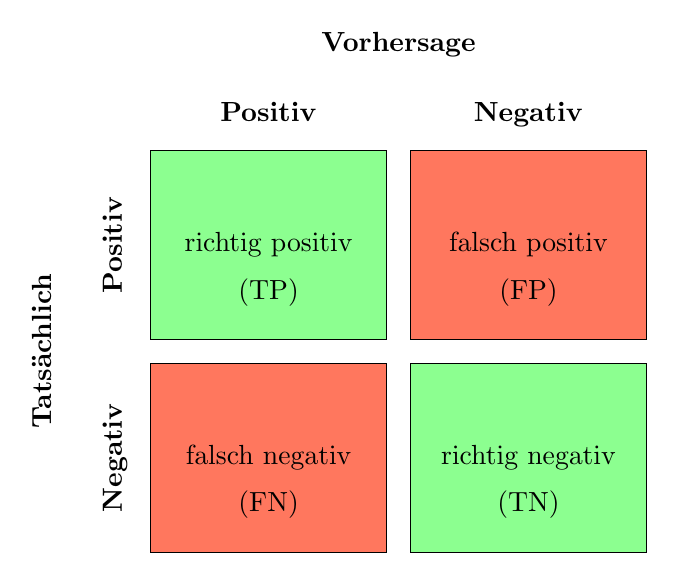
\begin{tikzpicture}[x = 3mm, y = 3mm]   % das hier verändern zum Skalieren
    % Bounding box
  \useasboundingbox (-5.2, -0.1) rectangle (21.2, 22.2);
  % links unten
  \filldraw [draw = black, fill = myRed] (0, 0) rectangle ++(10, 8);
  \tikztextc{5}{4}{falsch negativ}
  \tikztextc{5}{2}{(FN)}
  % rechts unten
  \filldraw [draw = black, fill = myGreen] (11, 0) rectangle ++(10, 8);
  \tikztextc{16}{4}{richtig negativ}
  \tikztextc{16}{2}{(TN)}
  % links oben
  \filldraw [draw = black, fill = myGreen!] (0, 9) rectangle ++(10, 8);
  \tikztextc{5}{13}{richtig positiv}
  \tikztextc{5}{11}{(TP)}
  % rechts oben
  \filldraw [draw = black, fill = myRed] (11, 9) rectangle ++(10, 8);
  \tikztextc{16}{13}{falsch positiv}
  \tikztextc{16}{11}{(FP)}
  % daneben
  \tikztextupc{-1.5}{4}{\textbf{Negativ}}
  \tikztextupc{-1.5}{13}{\textbf{Positiv}}
  \tikztextupc{-4.5}{8.5}{\textbf{Tatsächlich}}
  % drüber
  \tikztextc{5}{18.5}{\textbf{Positiv}}
  \tikztextc{16}{18.5}{\textbf{Negativ}}
  \tikztextc{10.5}{21.5}{\textbf{Vorhersage}}
 \end{tikzpicture}
 \caption{Konfusionsmatrix}
 \label{fig:konfusionsmatrix}
\end{figure}